\documentclass[tikz,border=5pt]{standalone}
\usepackage{tikz}
\usetikzlibrary{arrows.meta,decorations.pathmorphing,patterns}

% Atlas color palette
\definecolor{AtlasTeal}{HTML}{5BA4A4}
\definecolor{AtlasWarm}{HTML}{C17F59}
\definecolor{AtlasSage}{HTML}{7A9E7E}
\definecolor{AtlasWarmLight}{HTML}{F0DED3}

\begin{document}
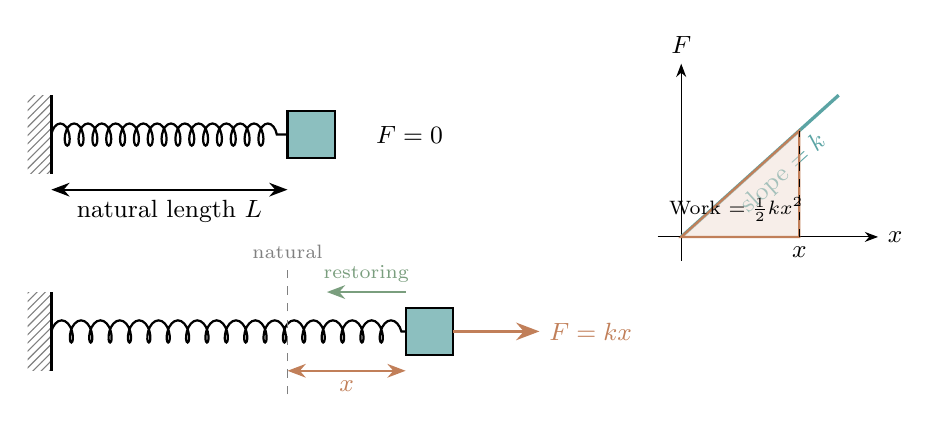
\begin{tikzpicture}[>=Stealth]
    
    % ========== TOP: Natural length ==========
    \begin{scope}[shift={(0,2.5)}]
        % Wall
        \fill[pattern=north east lines, pattern color=gray] (-0.3,-0.5) rectangle (0,0.5);
        \draw[very thick] (0,-0.5) -- (0,0.5);
        
        % Spring at natural length
        \draw[thick, decorate, decoration={coil, amplitude=4pt, segment length=5pt}] 
            (0,0) -- (3,0);
        
        % Block
        \fill[AtlasTeal!70] (3,-0.3) rectangle (3.6,0.3);
        \draw[thick] (3,-0.3) rectangle (3.6,0.3);
        
        % Natural length marker
        \draw[<->, thick] (0,-0.7) -- node[below, font=\small] {natural length $L$} (3,-0.7);
        
        % Label
        \node[right, font=\small] at (4, 0) {$F = 0$};
    \end{scope}
    
    % ========== BOTTOM: Stretched ==========
    \begin{scope}[shift={(0,0)}]
        % Wall
        \fill[pattern=north east lines, pattern color=gray] (-0.3,-0.5) rectangle (0,0.5);
        \draw[very thick] (0,-0.5) -- (0,0.5);
        
        % Spring stretched
        \draw[thick, decorate, decoration={coil, amplitude=4pt, segment length=7pt}] 
            (0,0) -- (4.5,0);
        
        % Block
        \fill[AtlasTeal!70] (4.5,-0.3) rectangle (5.1,0.3);
        \draw[thick] (4.5,-0.3) rectangle (5.1,0.3);
        
        % Extension x
        \draw[<->, thick, AtlasWarm] (3,-0.5) -- node[below, font=\small] {$x$} (4.5,-0.5);
        
        % Original position marker
        \draw[dashed, gray] (3,-0.8) -- (3,0.8);
        \node[above, font=\scriptsize, gray] at (3,0.8) {natural};
        
        % Force arrow
        \draw[->, very thick, AtlasWarm] (5.1,0) -- (6.2,0);
        \node[right, font=\small, AtlasWarm] at (6.2,0) {$F = kx$};
        
        % Restoring force arrow
        \draw[->, thick, AtlasSage] (4.5,0.5) -- (3.5,0.5);
        \node[above, font=\scriptsize, AtlasSage] at (4,0.5) {restoring};
    \end{scope}
    
    % ========== Graph (right side) ==========
    \begin{scope}[shift={(8,1.2)}]
        % Axes
        \draw[->] (-0.3,0) -- (2.5,0) node[right, font=\small] {$x$};
        \draw[->] (0,-0.3) -- (0,2.2) node[above, font=\small] {$F$};
        
        % Hooke's law line
        \draw[AtlasTeal, very thick] (0,0) -- (2,1.8);
        
        % Slope annotation
        \node[AtlasTeal, font=\small, rotate=42] at (1.3,0.8) {slope $= k$};
        
        % Work = area under curve
        \fill[AtlasWarmLight, opacity=0.5] (0,0) -- (1.5,0) -- (1.5,1.35) -- (0,0);
        \draw[AtlasWarm, thick] (0,0) -- (1.5,0) -- (1.5,1.35) -- cycle;
        
        \node[font=\scriptsize] at (0.7,0.35) {Work $= \frac{1}{2}kx^2$};
        
        % x marker
        \draw[dashed] (1.5,0) -- (1.5,1.35);
        \node[below, font=\small] at (1.5,0) {$x$};
    \end{scope}

\end{tikzpicture}
\end{document}
